%%%%%%%%%%%%%%%%%%%%%%%%%%%%%%%%%%%%%%%%%%%%%%%%%%%%%%%%%%%%%%%%%
% Contents : The categories chapter
% $Id : grisbi-manuel-categories.tex, v 0.4 2002/10/27 Daniel Cartron
% $Id : grisbi-manuel-categories.tex, v 0.5.0 2004/06/01 Loic Breilloux
% some of its content was in tips chapter : 
% $Id : grisbi-manuel-tips.tex, v 0.4 2002/10/27 Daniel Cartron
% $Id : grisbi-manuel-categories.tex, v 0.6.0 2011/11/17 Jean-Luc Duflot
% some of its content was in tips chapter :
% $Id : grisbi-manuel-tips.tex, v 0.5.0 2004/06/01 Loic Breilloux
% $Id : grisbi-manuel-categories.tex, v 0.8.9 2012/04/27 Jean-Luc Duflot
% $Id : grisbi-manuel-categories.tex, v 1.0 2014/02/12 Jean-Luc Duflot
%%%%%%%%%%%%%%%%%%%%%%%%%%%%%%%%%%%%%%%%%%%%%%%%%%%%%%%%%%%%%%%%%

\chapter{Catégories\label{categories}}


Pour pouvoir retrouver facilement les opérations, on les classe par catégories, par exemple \og Maison \fg{}, \og Remboursement \fg{}, qui peuvent éventuellement contenir des sous-catégories. En termes de comptabilité, il s'agit d'imputation comptable. Ne pas confondre avec le tiers, qui est celui avec qui on a la relation financière (un fournisseur ou un client).

Grisbi vous permet de faire la distinction entre les imputations comptables et les imputations budgétaires. Mais uniquement si vous le souhaitez.

Une imputation comptable, nommée \menu{Catégorie} dans Grisbi, définit la nature de  l'opération : frais de transport, loisirs, etc. Tandis qu'une imputation budgétaire définit la fonction de l'opération : il s'agit du travail, de la vie courante, des vacances, d'un projet d'aménagement, etc. D'une autre manière, \emph{quoi} et \emph{pourquoi}\ldots{ } Voir aussi le chapitre \vref{budgetarylines}, \menu{Imputations budgétaires}.

 espace pour changement de thème
\vspacepdf{5mm}
Après son installation, Grisbi propose par défaut une liste de catégories. Vous pouvez l'utiliser telle quelle, la modifier selon vos besoins en ajoutant ou en supprimant des catégories ou des sous-catégories, ou bien importer ou exporter une autre liste générée auparavant par Grisbi. Les noms de fichier de ces listes ont pour \indexword{extension} \file{.cgsb} \index{extension !.cgsb}\index{cgsb}, par exemple \file{mes-categories.cgsb}.

% espace avant Attention ou Note  : 5 mm
\vspacepdf{5mm}
\textbf{Note} : toutes vos opérations doivent être affectées à une catégorie \emph{et} à une sous-catégorie, pour deux raisons : elles pourront ainsi être bien classées, donc facilement gérées, et de plus, si elles ne sont pas affectées, elles ne pourront pas être prises en compte dans les budgets prévisionnels.

% espace avant Attention ou Note  : 5 mm
\vspacepdf{5mm}
\textbf{Note} : Il est donc conseillé de bien étudier votre liste de catégories, pour éviter d'avoir à la modifier fréquemment pour cause d'incohérences ou de redondances. Si vous avez vraiment des opérations inclassables, créez une catégorie ou des sous-catégories \og Divers \fg{}, mais n'abusez pas de leur emploi.

% espace pour changement de thème
\vspacepdf{5mm}
L'onglet \menu{Catégories} sert à gérer  toutes les catégories et sous-catégories de votre fichier de comptes.

Pour avoir accès à la gestion des catégories, sélectionnez \menu{Catégories} dans le panneau de navigation ou avec la barre d'information (voir le chapitre \vref{home}, \menu{Accueil}).

La barre d'information affiche, à gauche, le nom de la catégorie et de la sous-catégorie sélectionnées dans le pavé des détails et, complètement à droite, le solde des opérations affectées à la catégorie ou la sous-catégorie sélectionnée.

Le pavé des détails affiche deux éléments :
\begin{itemize}
	 \item la barre d'outils ;
	 \item la liste des catégories.
\end{itemize}


\section{Barre d'outils\label{categories-functions}}


La barre d'outils des catégories présente les fonctions suivantes  :

\begin{itemize}
	 \item \menu{Nouvelle catégorie} : ouvre une fenêtre pour créer une nouvelle catégorie ;
	 \item \menu{Nouvelle sous-catégorie} : ouvre une fenêtre pour créer une 	nouvelle sous-catégorie ;
	 \item \menu{Importer} : permet d'importer une liste de catégories contenue dans un fichier ;
	 \item \menu{Exporter} : permet d'exporter une liste de catégories dans un fichier ;
	 \item \menu{Supprimer} : supprime la catégorie ou la sous-catégorie sélectionnée ;
	 \item \menu{Éditer} : ouvre une fenêtre pour modifier le nom de la catégorie ou de la sous-catégorie sélectionnée ;
	 \item \menu{Affichage} : ouvre un menu déroulant pour afficher la liste des catégories, avec ou sans leurs sous-catégories.
\end{itemize}

La barre d'outils peut être déplacée dans l'écran en cliquant sur sa poignée (petit rectangle vertical à gauche de la barre) et en la déplaçant. Pour la réattacher à son emplacement d'origine dans le pavé des détails, la remettre en haut de la fenêtre, le haut de la poignée placé sur le petit trait qui visualise sa place d'origine.


\section{Liste des catégories et des sous-catégories\label{categories-list}}


La liste des catégories et sous-catégories s'affiche dans le panneau des \ifIllustration détails\refimage{categories-list-img}.
\else détails.
\fi

\ifIllustration
% image centrée
\begin{figure}[htbp]
\begin{center}
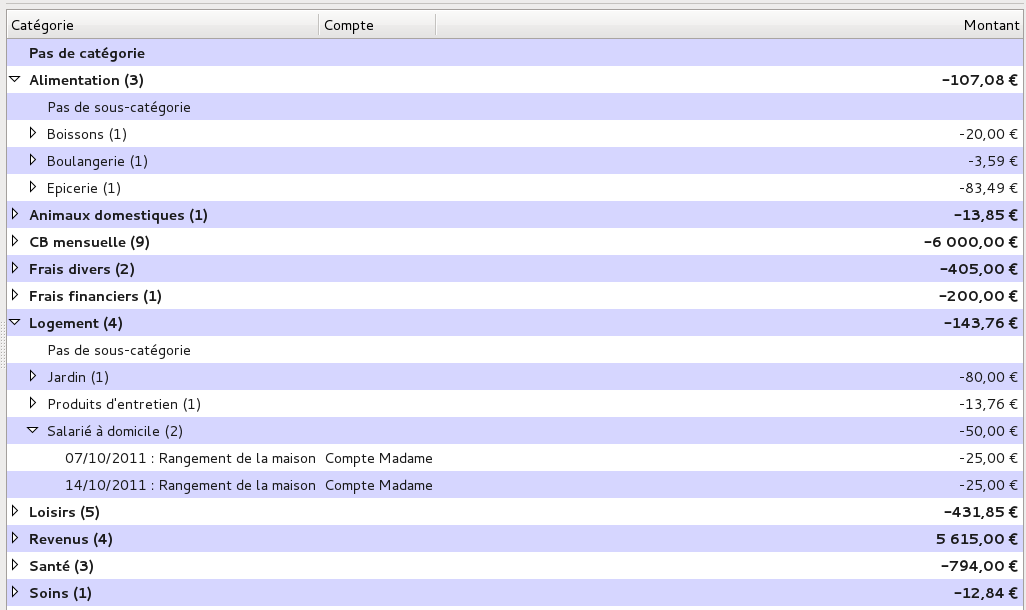
\includegraphics[scale=0.5]{image/screenshot/categories_list.png}
\end{center}
\caption{Liste des catégories et des sous-catégories}
\label{categories-list-img}
\end{figure}
% image centrée
\fi

Elle affiche en haut la barre des libellés des colonnes ; ses champs d'affichage sont les suivants :
\begin{itemize}
	 \item le nom de la catégorie ou de la sous-catégorie ;
	 \item le compte concerné ;
	 \item le montant total des opérations affectées aux  catégories et sous-catégories, et le montant de chaque opération affectée à ces catégories ou sous-catégories si leurs lignes sont déroulées.
\end{itemize}

Vous pouvez déplacer la liste des catégories vers le haut ou vers le bas avec la molette de la souris, ou bien avec la souris et l'ascenseur vertical. Le déplacement éventuel vers la gauche ou la droite se fait avec la souris et l'ascenseur horizontal.

Pour  \indexword{afficher les sous-catégories}\index{affichage !sous-catégories} d'une catégorie, cliquez sur le petit triangle à gauche de son nom, ou bien double-cliquez sur sa ligne ;
% ou bien sélectionnez-la et appuyez sur la barre d'espace (non fonctionnel) 
 cela affiche le libellé  de toutes les sous-catégories, et éventuellement, en première position, \indexword{\menu{Pas de sous-catégorie}}\index{sous-catégories !pas de sous-catégorie}.

\textbf{Note} : ces triangles peuvent être remplacés, en fonction du thème de l'environnement de bureau ou du gestionnaire de fenêtres que vous utilisez, par d'autres caractères tels que +, -, >, <, etc. 

%le seul moyen de dérouler la liste est de cliquer sur le petit triangle. il devrait y avoir un moyen avec le clavier, comme ça existe avec le formulaire de saisie, où l'on peut utiliser la barre d'espace pour le moyen de paiement, ou la touche flèche bas pour la catégorie...

% espace pour changement de thème
\vspacepdf{5mm}
Vous pouvez afficher plusieurs \indexword{catégories déroulées}\index{catégories !déroulées}. Pour ne plus les afficher, \indexword{enroulez les catégories}\index{catégories !enroulées} en cliquant sur le petit triangle à gauche de leur nom, ou bien double-cliquez sur leur ligne. Vous pouvez aussi dérouler ou enrouler toutes les catégories de la liste, en cliquant sur l'outil \menu{Affichage} dans la barre d'outils et en choisissant \menu{Vue des catégories et des sous-catégories}. Pour \indexword{afficher seulement les catégories}\index{affichage !catégories}, cliquez sur l'outil \menu{Affichage} dans la barre d'outils et choisissez \menu{Vue des catégories uniquement}.

Les catégories et sous-catégories de votre fichier de comptes sont affichées par ordre alphabétique, avec deux exceptions : la première catégorie affichée est toujours la catégorie de libellé \indexword{\menu{Pas de catégorie}}\index{catégories !pas de catégorie}, qui reçoit toutes les opérations dont la catégorie n'est pas définie, et, à l'intérieur d'une catégorie, la première sous-catégorie affichée est toujours la sous-catégorie de libellé \indexword{\menu{Pas de sous-catégorie}}\index{sous-catégories !pas de sous-catégorie}, qui reçoit toutes les opérations dont la sous-catégorie n'est pas définie.

Le nombre d'opérations affectées à chaque catégorie ou sous-catégorie s'affiche, entre parenthèses, à la suite de son nom, et le montant total des opérations affectées à ces catégories ou sous-catégories s'affiche dans la colonne \menu{Montant}, à droite sur la même ligne. 

% Bogue connu  : en cliquant sur une ligne de catégories, la barre d'information devrait afficher le total, mais n'affiche que 0. 

% espace avant Attention ou Note  : 5 mm
\vspacepdf{5mm}
\textbf{Note} : vous pouvez configurer la \indexword{devise des totaux}\index{devise !totaux} de toutes les (sous-) catégories dans le menu \menu{Édition - Préférences} (voir la section \vref{setup-display-third-currencies}, \menu{Devises des totaux}).


\section{Sélection d'une catégorie ou d'une sous-catégorie\label{categories-selection}}


Pour sélectionner une catégorie ou une sous-catégorie, vous avez deux moyens :

\begin{itemize}
	 \item cliquez sur sa ligne ;
	 \item déplacez la sélection avec les touches du clavier \key{Flèche Haut}, \key{Flèche Bas}, \key{Page Haut} ou \key{Page Bas}.
\end{itemize}

Le nom de la catégorie ou sous-catégorie apparaît alors sur fond rose{\couleur}.

% espace pour changement de thème
\vspacepdf{5mm}
Un menu contextuel est disponible par un clic-droit sur la liste des catégories ; selon la ligne sélectionnée, vous pouvez exécuter les fonctions suivantes :

\begin{itemize}
	 \item pour une catégorie : \menu{Éditer la catégorie sélectionnée} ;
	 \item pour la sous-catégorie \menu{Pas de sous-catégorie} :
		\begin{itemize}
			 \item si elle est vide : \menu{Éditer la catégorie sélectionnée},
			 \item si elle contient des opérations : \menu{Transférer les opérations dans une autre sous-catégorie},
		\end{itemize}
	 \item pour	une sous-catégorie quelconque :	
		\begin{itemize}
			 \item \menu{Éditer la sous-catégorie sélectionnée},
			 \item \menu{Gérer les sous-catégories},			 
		\end{itemize}		
	 \item pour une opération quelconque : \menu{Transférer des opérations identiques dans une autre sous-catégorie}.	
\end{itemize}

\ifIllustration
% saut de page pour titre solidaire
\newpage
\fi


\section{Les opérations d'une catégorie ou d'une sous-catégorie\label{categories-transactions}}


Une ligne de libellé \menu{Pas de sous-catégorie} se comporte exactement comme une ligne de libellé de sous-catégorie.

Pour afficher les opérations, cliquez sur le petit triangle à gauche du libellé  \menu{Pas de sous-catégorie} ou celui d'une sous-catégorie, ou bien double-cliquez sur sa ligne,
% ou bien sélectionnez-la et appuyez sur la barre d'espace (non fonctionnel),
 ce qui déroule la liste. Les opérations sont alors décrites sur une seule ligne, avec leur date, leur remarque éventuelle, le nom du compte concerné et leur montant.

\textbf{Note} : ces triangles peuvent être remplacés, en fonction du thème de l'environnement de bureau ou du gestionnaire de fenêtres que vous utilisez, par d'autres caractères tels que +, -, >, <, etc. 

%le seul moyen de dérouler la liste est de cliquer sur le petit triangle. il devrait y avoir un moyen avec le clavier, comme ça existe avec le formulaire de saisie, où l'on peut utiliser la barre d'espace pour le moyen de paiement, ou la touche flèche bas pour la catégorie...
 
% espace pour changement de thème
\vspacepdf{5mm}
Vous pouvez afficher plusieurs lignes de \indexword{sous-catégories déroulées}\index{sous-catégories !déroulées}. Pour ne plus les afficher, \indexword{enroulez les opérations}\index{sous-catégories !enroulées} d'une sous-catégorie en cliquant sur le petit triangle à gauche de leur nom, ou bien double-cliquez sur leur ligne. Vous pouvez aussi dérouler ou enrouler toutes les opérations de toutes les catégories et sous-catégories de la liste, en cliquant sur l'outil \menu{Affichage} dans la barre d'outils, et en faisant votre choix entre \menu{Vue des catégories uniquement}, \menu{Vue des catégories et sous-catégories} ou \menu{Vue complète}.

%espace pour changement de thème
\vspacepdf{5mm}
Vous pouvez \indexword{déplacer une opération}\index{sous-catégories !déplacement d'opération} d'une sous-catégorie vers une autre sous-catégorie de la liste (mais pas à partir de \menu{Pas de catégorie} ni vers \menu{Pas de catégorie}) en sélectionnant cette opération et en faisant un glisser-déplacer sur la sous-catégorie cible, exactement à l'endroit où son nom est entouré d'une bordure pointillée.

%espace pour changement de thème
\vspacepdf{5mm}
Un \indexword{double-clic} sur une ligne d'opération d'une catégorie\index{catégories !double-clic sur opération} ou d'une sous-catégorie\index{sous-catégories !double-clic sur opération} ferme l'onglet \menu{Catégories}, ouvre l'onglet \menu{Comptes} et le sous-onglet du compte contenant cette opération, sélectionne l'opération concernée et l'affiche dans le formulaire de saisie. De cette façon, cette opération peut être affichée et modifiée facilement.


\section{Création d'une catégorie ou d'une sous-catégorie\label{categories-new}}


\ifIllustration
% image entourée par un paragraphe ( picins)
% Pas de référence à l'illustration car erreur de numéro de figure avec picins.
\pichskip{8mm}
% supprimé car en html les figures entourées ne sont pas numérotées, et la numérotation des figures centrées décalée par rapport au pdf
%\piccaption{Création d'une  catégorie (ou d'une sous-catégorie)}
\label{categories-new-img}
\parpic[r]{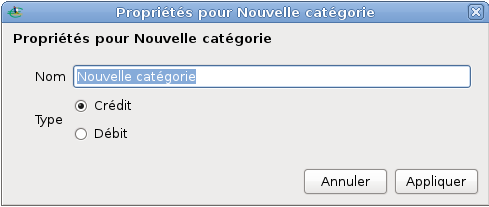
\includegraphics[scale=0.5]{image/screenshot/categories_new.png}}
% image entourée par un paragraphe ( picins)
\fi

La façon la plus immédiate pour créer une catégorie ou une sous-catégorie est de saisir son nom pendant la création d'une nouvelle opération dans l'onglet des comptes (voir la section \vref{transactions-fillcombo}, \menu{Nouveau tiers, catégorie ou imputation budgétaire}) ; mais vous pouvez aussi en créer ici, en cliquant sur l'outil \menu{Nouvelle catégorie} ou \menu{Nouvelle sous-catégorie}. Une boîte de dialogue s'ouvre ; suivant le cas, renseignez le nom de la catégorie et cochez si elle contiendra des crédits ou des débits, ou renseignez uniquement le nom de la sous-catégorie, puis validez.

% espace pour changement de thème
\vspacepdf{5mm}
L'outil \menu{Nouvelle sous-catégorie}\label{categories-newsub} de la barre d'outils ne devient actif que lorsqu'une catégorie est sélectionnée dans la liste.

\ifIllustration
% saut de page pour titre solidaire
\newpage
% espace après image entourée
\vspacehevea{5mm}
\fi


\section{Modification d'une catégorie ou d'une sous-catégorie\label{categories-modify}}


Pour modifier une catégorie ou une sous-catégorie, procédez comme suit :
% espace avant image 5mm
\vspacepdf{3mm}

\begin{enumerate}	
	\ifIllustration
	% image entourée par un paragraphe ( picins)
	% Pas de référence à l'illustration car erreur de numéro de figure avec picins.
	\pichskip{8mm}
	% supprimé car en html les figures entourées ne sont pas numérotées, et la numérotation des figures centrées décalée par rapport au pdf
%	\piccaption{Modification d'une catégorie}
	\label{categories-infos-img}
	\parpic[r]{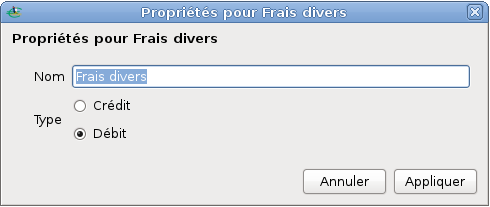
\includegraphics[scale=0.51]{image/screenshot/categories_infos}}
	% image entourée par un paragraphe ( picins)
	\fi
	 \item sélectionnez sa ligne ;
	 \item cliquez sur l'outil \menu{Éditer} dans la barre d'outils, ou sélectionnez \menu{Éditer la catégorie sélectionnée} ou \menu{Éditer la sous-catégorie sélectionnée} dans le menu contextuel accessible par un  clic-droit ;
	 \item une boîte de dialogue s'affiche : modifiez son nom et, seulement pour les catégories, son type (crédit ou débit) ;
	 \item validez.
\end{enumerate}


\textbf{Note} : la sous-catégorie \menu{Pas de sous-catégorie} est créée automatiquement par Grisbi ; vous ne pouvez pas la modifier.


\section{Transfert d'opérations dans une autre sous-catégorie\label{categories-transfer}}

Vous pouvez \indexword{transférer des opérations dans une autre sous-catégorie}\index{sous-catégories !transfert d'opérations} ayant pour point commun soit le tiers, soit la remarque, soit les deux ; pour cela, procédez comme suit :
% espace avant image 5mm
\vspacepdf{3mm}

\begin{enumerate}
	\ifIllustration
	% image entourée par un paragraphe ( picins)
	% Pas de référence à l'illustration car erreur de numéro de figure avec picins.
	\pichskip{8mm}
	% supprimé car en html les figures entourées ne sont pas numérotées, et la numérotation des figures centrées décalée par rapport au pdf
	%\piccaption{Transfert d'opérations identiques dans une autre sous-catégorie}
	\label{categories_transfer-img}
	\parpic[r]{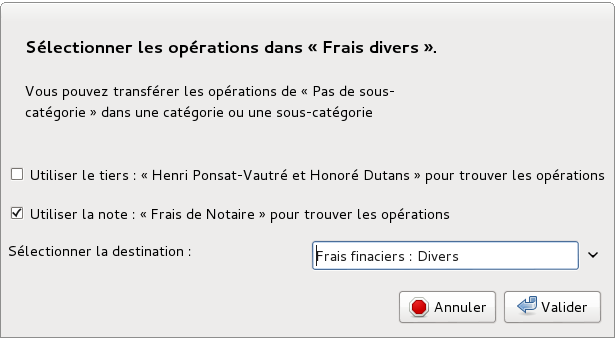
\includegraphics[scale=0.51]{image/screenshot/categories_transfer}}
	% image entourée par un paragraphe ( picins)
	\fi
	
	 \item sélectionnez la ligne de l'opération concernée ;
	 \item sélectionnez \menu{Transférer des opérations identiques dans une autre sous-catégorie}, dans le menu contextuel accessible par un  clic-droit ;
	 \item une boîte de dialogue s'affiche ; cochez l'une des deux cases \menu{Utiliser le tiers\ldots{ }} et \menu{Utiliser la note\ldots{ }} ou les deux selon votre besoin ;
	 \item renseignez le champ libellé \menu{Sélectionner la destination}, ou choisissez une catégorie et une sous-catégorie dans la liste déroulante ;
	 \item validez.
\end{enumerate}

\textbf{Note} : la saisie du champ de libellé \menu{Sélectionner la destination} bénéficie de la fonction d'\indexword{auto-complètement}\index{champ de saisie !auto-complètement}.

\ifIllustration
% espace après image entourée
\vspacehevea{15mm}
\fi

\section{Gestion des sous-catégories\label{categories-management}}


Vous pouvez modifier l'organisation de vos sous-catégories en \indexword{déplaçant le contenu d'une sous-catégorie}\index{sous-catégories !déplacement d'opération} vers une autre ou vers une nouvelle catégorie. Pour cela, sélectionnez une sous-catégorie, puis cliquez-droit et choisissez dans le menu contextuel \ifIllustration \refimage{categories-management-img} :
\else  :
\fi

\begin{itemize}
	 \item pour une sous-catégorie \menu{Pas de sous-catégorie} non vide : sélectionnez  \menu{Transférer les opérations dans une autre sous-catégorie} : une fenêtre s'affiche ; sélectionnez la destination dans la liste déroulante, puis validez ;

	 \item pour les autres sous-catégories : sélectionnez \menu{Gérer les sous-catégories}, une fenêtre s'affiche ; sélectionnez l'action désirée  :
		\begin{itemize}
			 \item \menu{Transférer les opérations dans une catégorie ou une sous-catégorie} : sélectionnez la catégorie de destination dans la liste déroulante, puis validez,
			 \item \menu{Transférer \og nom de la sous-catégorie sélectionnée \fg{} dans une autre catégorie} : sélectionnez la catégorie de destination dans la liste déroulante, puis validez,
			 \item \menu{Convertir \og nom de la sous-catégorie sélectionnée \fg{} en nouvelle catégorie} : validez, la sous-catégorie est devenue une catégorie.
		\end{itemize}
\end{itemize}

\ifIllustration
% image centrée
\begin{figure}[htbp]
\begin{center}
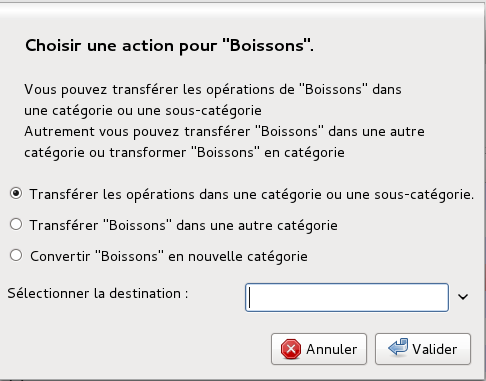
\includegraphics[scale=0.5]{image/screenshot/categories_management}
\end{center}
\caption{Gestion des sous-catégories}
\label{categories-management-img}
\end{figure}
% image centrée
\fi

%
\section{Suppression d'une catégorie ou d'une sous-catégorie\label{categories-delete}}


Pour supprimer une catégorie ou une sous-catégorie, procédez comme suit :
% espace avant image 5mm
\vspacepdf{3mm}

\begin{enumerate}
	\ifIllustration
	% image entourée par une liste (picins)
	% Pas de référence à l'illustration car erreur de numéro de figure avec picins.
	\pichskip{8mm}
	% supprimé car en html les figures entourées ne sont pas numérotées, et la numérotation des figures centrées décalée par rapport au pdf
	%\piccaption{Suppression d'une catégorie}
	\label{categories-delete-img}
	\parpic[r]{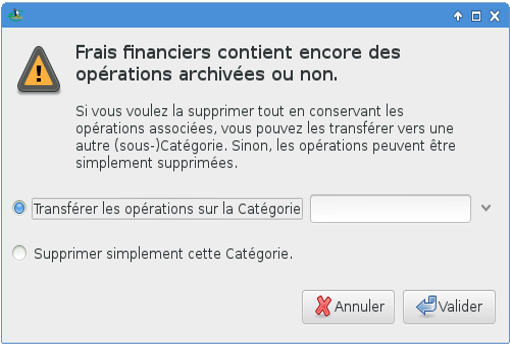
\includegraphics[scale=0.5]{image/screenshot/categories_delete}}
	% image entourée par une liste (picins)
	\fi
	 \item sélectionnez-la dans la liste ;
	 \item cliquez sur l'outil \menu{Supprimer} dans la barre d'outils ;
	 \item une  boîte de dialogue s'ouvre et vous propose soit de réaffecter les opérations de cette (sous-) catégorie vers une autre (sous-) catégorie, soit de la supprimer purement et simplement, y compris toutes ses opérations ;
	 \item faites votre choix puis validez.
\end{enumerate}


\ifIllustration
% espace après légende 10mm
\vspacepdf{9mm}
\fi

\strong{Attention} : la suppression d'une catégorie ou d'une sous-catégorie est \indexword{irréversible}\index{opération !irréversible} !

% espace avant Attention ou Note  : 5 mm
\vspacepdf{5mm}
\textbf{Note} : si la (sous-) catégorie que vous voulez supprimer ne contient aucune opération, aucune boîte de dialogue ne s'ouvrira et Grisbi la supprimera immédiatement.

\ifIllustration
% espace après image entourée
\vspacehevea{20mm}
\fi


\section{Import et export\label{categories-importexport} }


Grisbi vous permet d'importer ou d'exporter les catégories d'un fichier de comptes, ce qui peut éviter de recréer tout un ensemble de catégories si on peut le trouver ailleurs déjà fait.


\subsection{Import d'une liste de (sous-) catégories\label{categories-importexport-import} }

Pour \indexword{importer une liste de (sous-) catégories}\index{catégories !import}\index{sous-catégories !import}, procédez comme suit :

\begin{enumerate}
	 \item cliquez sur l'outil \menu{Importer} dans la barre d'outils : une fenêtre de gestionnaire de fichiers s'affiche ;
	 \item choisissez le répertoire et le nom du fichier à importer, dont l'\indexword{extension} doit être \file{.cgsb}\index{extension !.cgsb}\index{cgsb} ;
	 \item cliquez sur le bouton \menu{Ouvrir} ; une boîte de dialogue vous demande de choisir entre deux options :
		    \begin{itemize}
			      \item fusion des catégories importées avec celles de votre fichier de comptes en cours d'utilisation (bouton \menu{Valider}),
			      \item remplacement des catégories de votre fichier de comptes en cours d'utilisation par les catégories importées (bouton \menu{Remplacer l'existant}) ;
		     \end{itemize}
	 \item cliquez sur le bouton de votre choix ; les nouvelles catégories sont enregistrées dans votre fichier de comptes, en plus de celles qui étaient déjà présentes.
\end{enumerate}

\strong{Attention} : d'une manière générale, il est déconseillé d'avoir des accents ou des espaces dans les noms des répertoires et fichiers utilisés par Grisbi. Si c'est le cas, renommez-les maintenant. Par exemple, les espaces peuvent être remplacées par des tirets bas (\_).

% espace après Attention ou Note  : 5 mm
\vspacepdf{5mm}
Quelle que soit l'option choisie, il vous appartient ensuite de supprimer une à une toutes les catégories que vous ne voulez pas garder, ou d'en créer de nouvelles.

% espace avant Attention ou Note  : 5 mm
\vspacepdf{5mm}
\textbf{Note} : si vous commencez un fichier de comptes neuf, vous aurez avantage à supprimer les catégories existantes par défaut avant d'importer une autre liste.


\subsection{Export de vos (sous-) catégories\label{categories-importexport-export} }

Pour \indexword{exporter la liste de vos (sous-) catégories}\index{catégories !export}\index{sous-catégories !export}, procédez comme suit :

\begin{enumerate}
	 \item cliquez sur l'outil \menu{Exporter} dans la barre d'outils : une fenêtre de gestionnaire de fichiers s'affiche ;
	 \item saisissez le nom du fichier à exporter, dont l'\indexword{extension} sera \file{.cgsb}\index{extension !.cgsb}\index{cgsb} ;
	 \item choisissez son répertoire de destination ;
	 \item cliquez sur le bouton \menu{Enregistrer}.
\end{enumerate}

% espace avant Attention ou Note  : 5 mm
\strong{Attention} : d'une manière générale, il est déconseillé d'avoir des accents ou des espaces dans les noms des répertoires et fichiers utilisés par Grisbi. Si c'est le cas, renommez-les maintenant. Par exemple, les espaces peuvent être remplacées par des tirets bas (\_).

%
%
%%\subsection{Format des fichiers de catégories}
%%
%%Ces fichiers sont enregistrés au format \file{XML}, comme le fichier de comptes.
%%La structure du fichier est identique à celle du fichier de comptes, section
%%\file{Categories} (voir l'annexe \vref{xml-categories}).